\casesection{Secondary flow at bends (sed-mor)}
\label{case:e02-f22-c29}
%------------------------------------------------------------------------------

\paragraph*{Purpose}

The purpose of this validation case is to examine the performance secondary flow  functionality in a bend or an arch shape channel flow simulation. The test case used is shown in figure \ref{fig:testcase_kalkwijkandBooij} and it is taken from Kalkwijk and Booij (1986). The test case number is e02-f22-c29.

\begin{figure}[h!]
	\begin{center}
		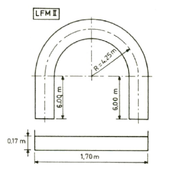
\includegraphics[width=0.5\columnwidth]{figures/testcasekalkwijkandBooij.png}
	\end{center}\caption{ A view of the case which is selected for validation purpose. It is taken from Kalkwijk and Booij (1986)-(LFM(II) channel)}
	\label{fig:testcase_kalkwijkandBooij}
\end{figure}

\paragraph*{Linked claims}
%\begin{itemize}
%	\item
The effect of secondary flow in flow patterns gives almost a similar result in Flexible Mesh compared to Delft3D4 software.
% almost the same result compare to Delft3D software. 
%\end{itemize} 
\paragraph*{Approach}
Three models have been setup: 
\begin{enumerate}
	\item specifying all the input and using D-Flow-sed-mor module of Delft3D 4.01 software.
	\item specifying all the input but using D-FLow-sed-mor module of Delft3D Flexible Mesh (structured grid).
	\item specifying all the input but using D-FLow-sed-mor module of Delft3D Flexible Mesh (unstructured grid).
\end{enumerate}

\paragraph*{Model description}
A simple structured and unstructured flexible mesh networks for the arch channel are built with the dimensions shown in \ref{fig:testcasekalkwijkandBooij}. Curvilinear grid also generated similar to FM-net as shown in \ref{fig:FMnet}. 

\begin{figure}[h!]
	\begin{center}
		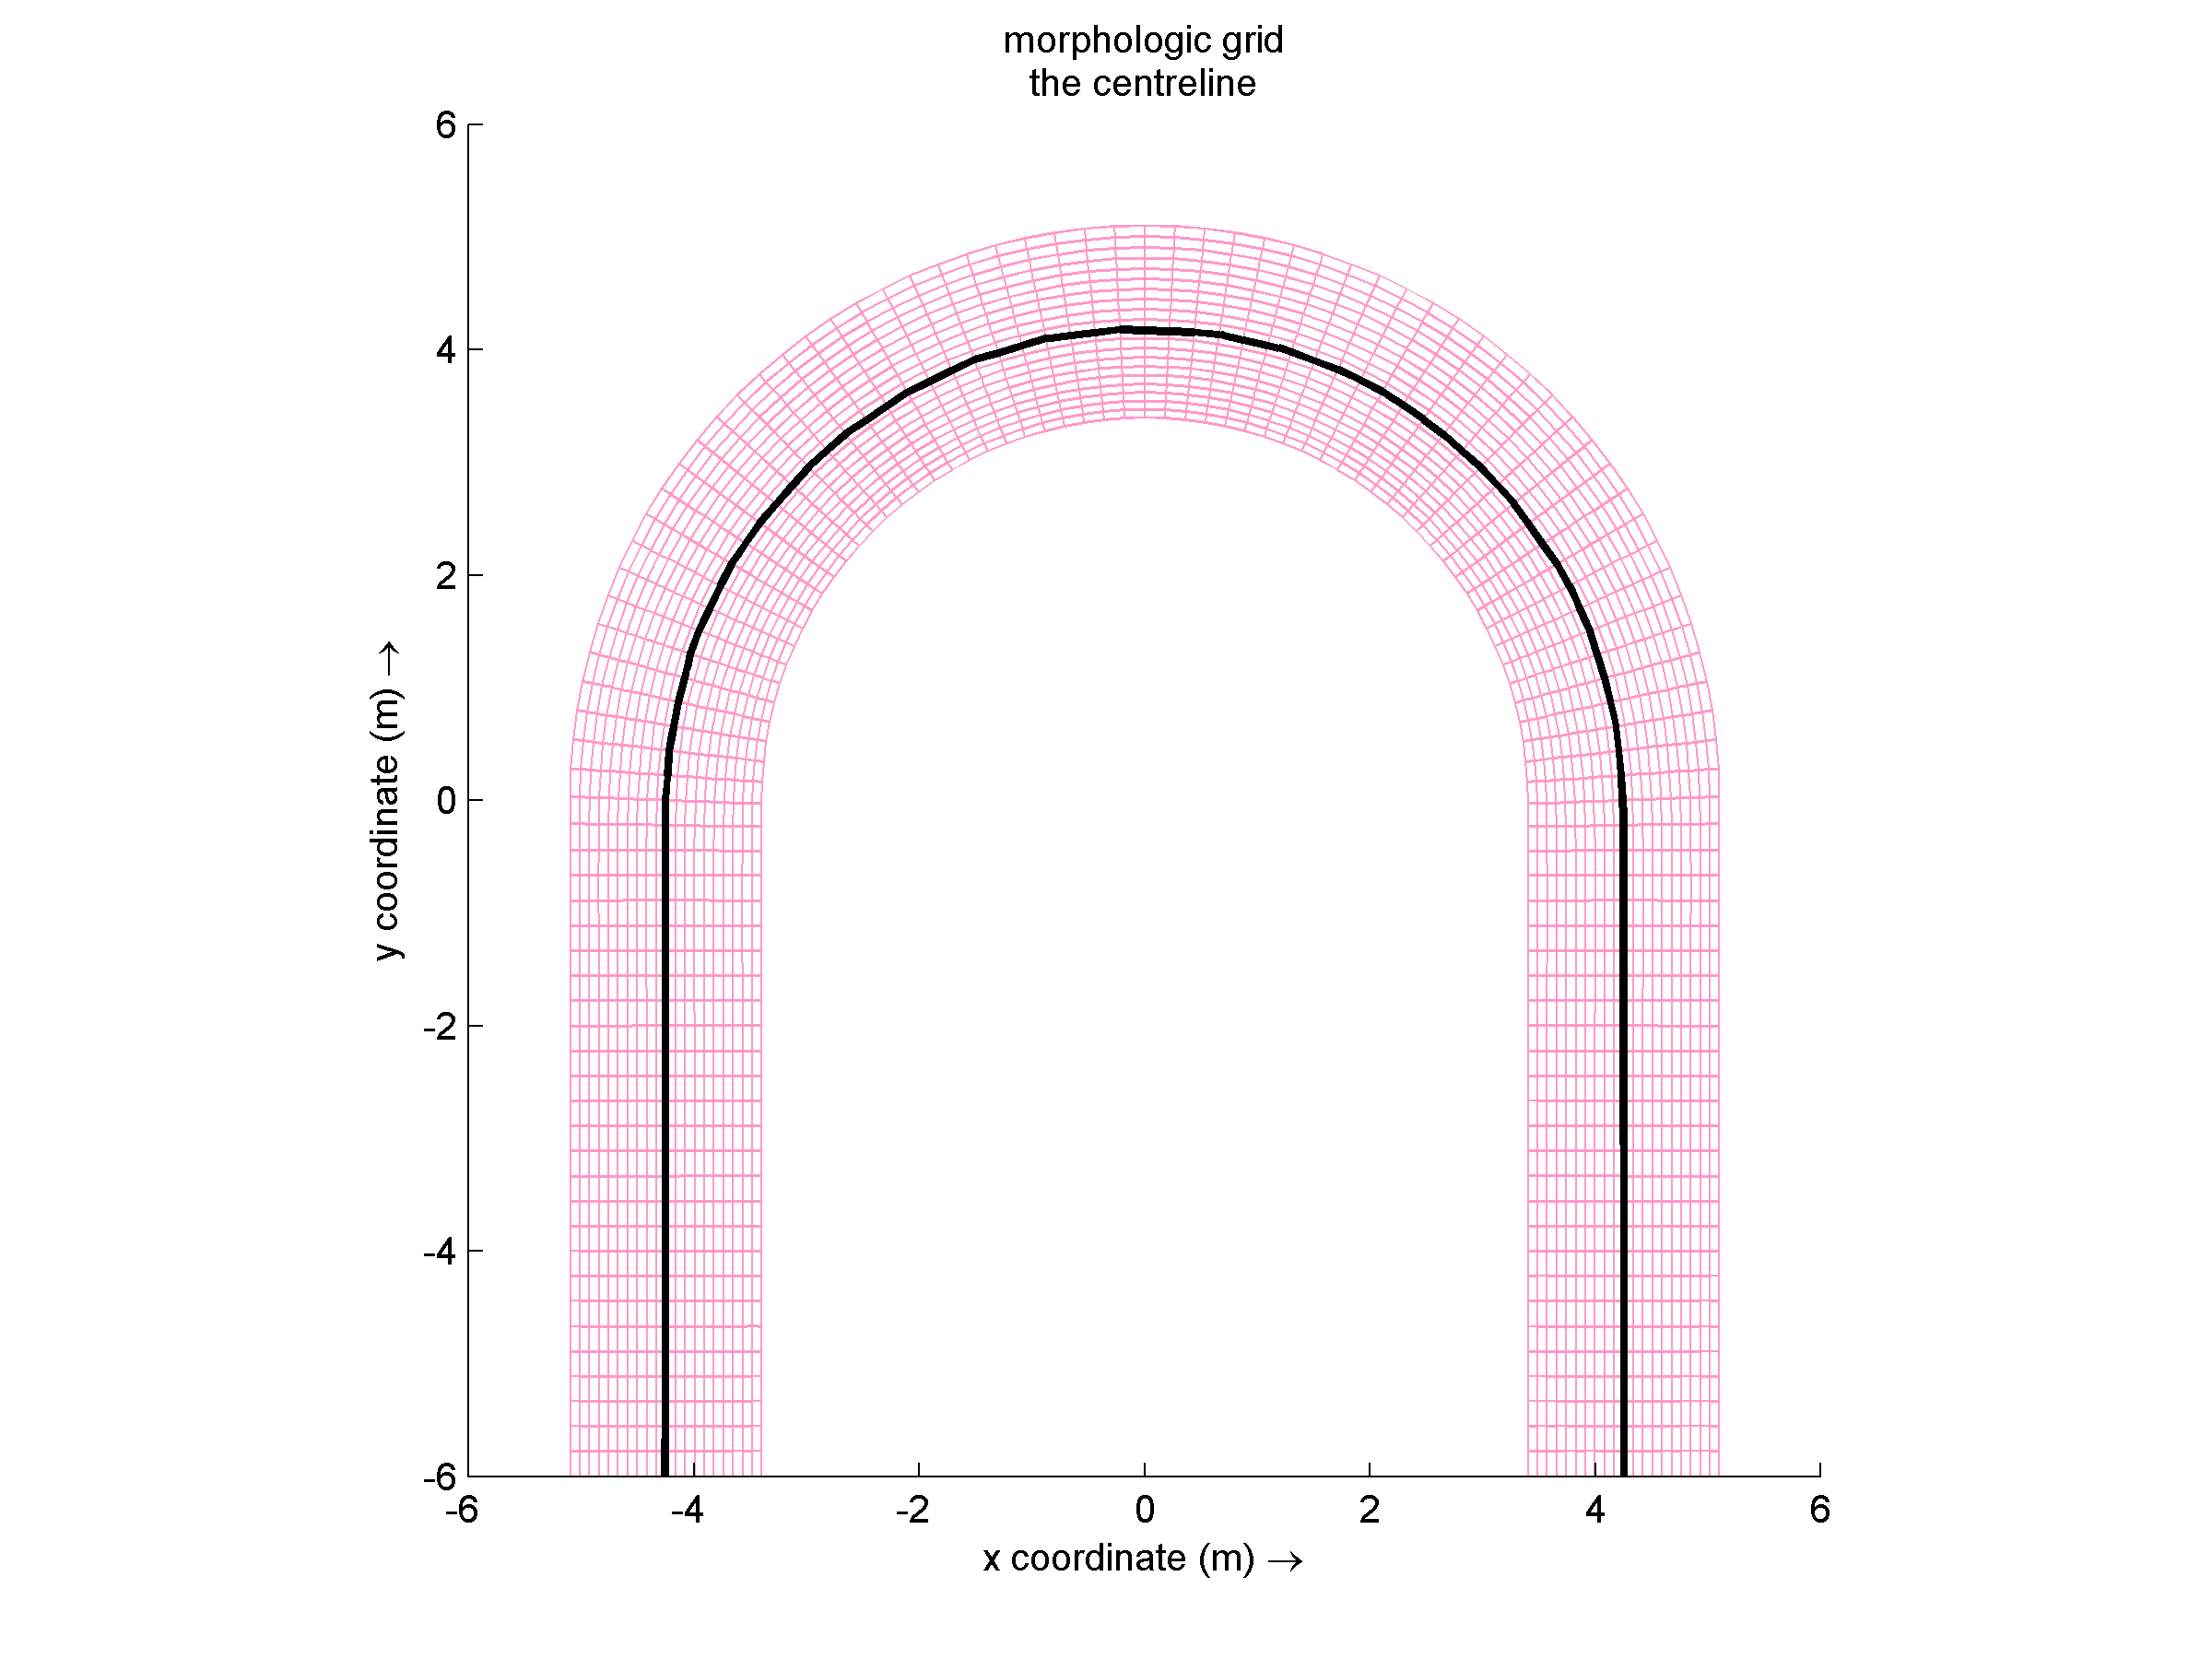
\includegraphics[width=1.0\columnwidth]{figures/FMnet.png}
	\end{center}\caption{The network used to test the coupling of secondary flow.}
	\label{fig:FMnet}
\end{figure}

The test cases concern LFM(II) channel flow with bed level of zero and a constant roughness factor under equilibrium flow conditions. A discharge $Q$ equal to 0.5 m$^3$/s is prescribed as upstream boundary condition. The longitudinal bottom slope $i_b$ is prescribed to be $0$. The Ch\'ezy friction coefficient $C$ is set to 60 m$^{1/2}$/s. The downstream boundary condition is water level set to 0.7 m.

\begin{figure}[h!]
	\begin{center}
		\includegraphics[width=1.0\columnwidth]{figures/C29Map2flowA.png}
	\end{center}\caption{Spiral flow intensity Map comparison (C29)}
	\label{fig:map}
\end{figure}
\begin{figure}[h!]
	\begin{center}
		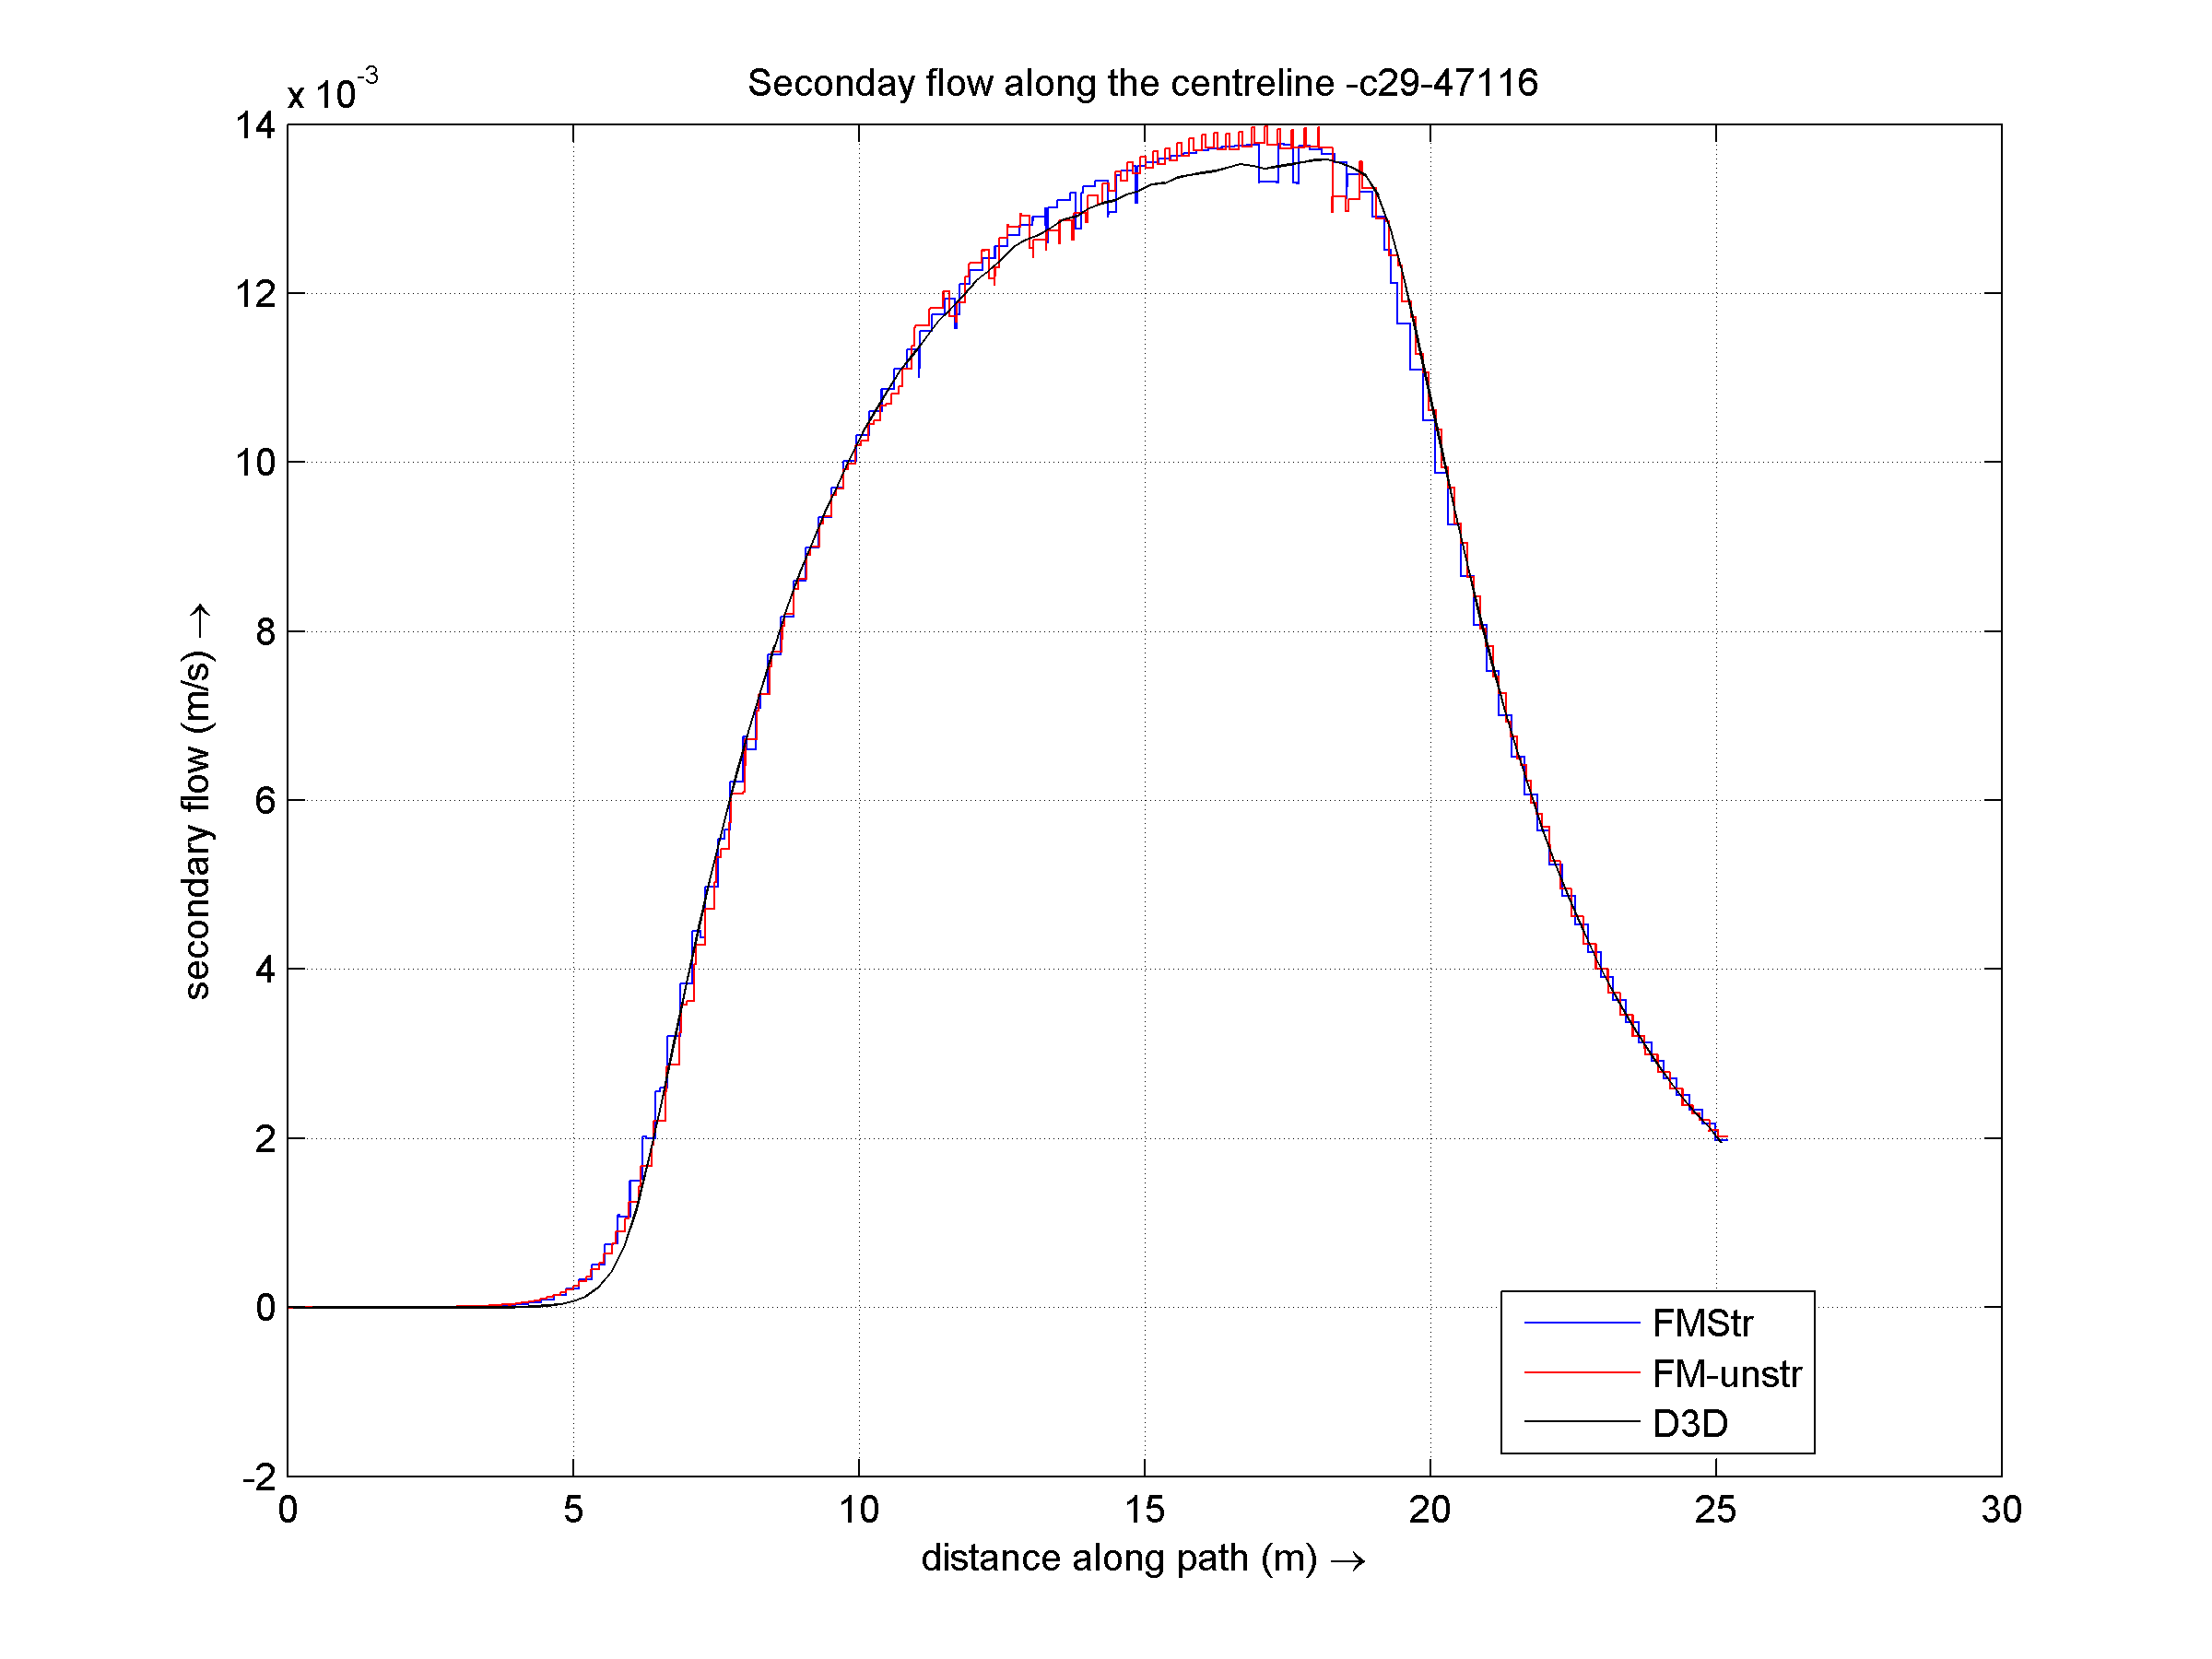
\includegraphics[width=1.0\columnwidth]{figures/C29Secondayflow-47116.png}
	\end{center}\caption{Bed load transport magnitude}
	\label{fig:line}
\end{figure}

\paragraph*{Results}

The results show that the secondary intensity and pattern are almost similar in structured and unstructured FM net as Delft3D4 (see figure \ref{fig:map} and \ref{fig:line}) .

\paragraph*{Conclusion}
The result shows that secondary flow in FM is similar as Delft3D4.
\paragraph*{Version}
This test has been carried out using the following software versions:
\begin{itemize}
	
	\item[$\bullet$] dflow-fm-x64-1.1.188.47116 - Flexible Mesh. 
	\item[$\bullet$] FLOW2D3D Version 6.02.07.6118 - Delft3D4
	
\end{itemize}

%------------------------------------------------------------------------------

